%% =========================================================================
%% Seeding metaheuristics for the Interval JSP: an anytime study of when
%% initialisation helps. Target: Swarm and Evolutionary Computation (Q1).
%% Draft v1.3 (2026-08-24): all sections written from the final data
%% (61 inst x 7 arms x 4 solvers x 30 runs = 51,240 runs, single protocol).
%% PENDING, requires input we do not have:
%%   - seed-generation times per generator (Sec. 4.3)
%%   - replication table for the appendix (Sec. 3.3)
%%   - FTOP sub-study outcome (Sec. 6.2), if it was ever run
%%   - optional: 2-3 further refs on RL-seeded metaheuristics (Sec. 2)
%%   - Data and code availability: Zenodo DOI + framework commit hash
%% =========================================================================
\documentclass[review]{elsarticle}

\usepackage{amsmath,amssymb}
\usepackage{graphicx}
\usepackage{booktabs}
\usepackage{multirow}

\journal{Swarm and Evolutionary Computation}

\begin{document}

\begin{frontmatter}

\title{Seeding metaheuristics with learned and heuristic solution pools for
the Interval Job Shop Scheduling Problem: an anytime study of when
initialisation helps}

\author[uniovi]{Hern\'an D\'iaz Rodr\'iguez}
\ead{herdiaz21@uniovi.es}

\affiliation[uniovi]{organization={Department of Computer Science, University of Oviedo},
            country={Spain}}

\begin{abstract}
Practitioners routinely assume that seeding the initial population of a
metaheuristic with good solutions improves its results. We test this
assumption rigorously on the Job Shop Scheduling Problem with interval
processing times (IJSP), using a portfolio of four published solvers that
spans the weak-to-strong search axis --- a genetic algorithm, an elitist
artificial bee colony, a memetic ABC with hill-climbing, and a
state-of-the-art tabu-search hybrid --- and five seed generators: a deep
reinforcement-learning policy and a quality ladder of randomised
constructive heuristics. A pilot study reveals three failure modes that
routinely corrupt seeding evaluations: stagnation-triggered early stopping,
budget-dependent apparent gains that reverse at convergence, and
self-referential measures of convergence speed. Our final design
pre-registers stopping rules, seeding fractions and decision criteria,
evaluates 61 interval Taillard instances with paired runs, and reports
final quality against published lower bounds, for which we establish a
validity argument specific to the interval setting. Over 51{,}240 runs the
effect of seeding proves not to be predicted by solver strength: a mixed
pool improves the weakest solver on 35 of 61 instances while losing on
none, leaves a memetic ABC unchanged, \emph{degrades} the genetic
algorithm, and improves the state-of-the-art tabu hybrid only on the
largest instances --- where, however, it does so decisively, and where
every generator we tested, including those harmful everywhere else, beats
the unseeded control. The governing variable is the ratio of instance size
to search budget rather than solver quality: 94.8\% of the aggregate gain
on the tabu hybrid comes from a single size class. At a tenth of the
budget, by contrast, seeding cuts the deviation from the lower bound by
28\% to 44\% on \emph{all four} solvers. We show that pool \emph{diversity}
rather than raw seed quality drives the gain, and that the negative result
on the genetic algorithm is an incompatibility with its position-preserving
crossover rather than the premature convergence usually invoked, which our
diversity measurements do not support.
\end{abstract}

\begin{keyword}
Job shop scheduling \sep interval uncertainty \sep population seeding \sep
metaheuristics \sep reinforcement learning \sep anytime behaviour
\end{keyword}

\end{frontmatter}

%% =========================================================================
\section{Introduction}\label{sec:intro}

Real-world scheduling rarely enjoys exact knowledge of task durations. When
only lower and upper bounds are available, the Job Shop Scheduling Problem
with interval processing times (IJSP) models each duration as a closed
interval and propagates interval arithmetic through the schedule
\cite{Lei2011,Lei2012}. The IJSP has accumulated a substantial algorithmic
literature over the last years, including genetic algorithms
\cite{DiazIPMU2020}, elitist artificial bee colony variants
\cite{DiazIWINAC2022,DiazESABC2023}, fast memetic ABC hybrids
\cite{DiazNatComp2023}, and, most recently, tabu-search hybrids built on
extreme-critical-path neighbourhoods that constitute the current state of
the art \cite{DiazTSN2}.

In parallel, learning-based methods have begun to produce fast constructive
policies for shop scheduling \cite{ZhangL2D2020,Bengio2021}. A deep
reinforcement-learning (RL) dispatching policy for the IJSP can emit
thousands of feasible, above-average solutions per instance in seconds,
raising an obvious question: should we seed the initial populations of
existing metaheuristics with such solutions? Folk wisdom answers yes, and
heuristic seeding of evolutionary algorithms has a long history
\cite{Kazimipour2014,Louis2004}. Yet the empirical evidence behind that
wisdom is weaker than it appears. Seeding studies typically compare final
objective values under a fixed stopping rule, and our pilot experiments
show that this practice is fragile in three specific ways.

First, \emph{stagnation-triggered stopping}: under the customary
``$N$ iterations without improvement'' rule, a well-seeded population that
the solver cannot immediately improve triggers the rule at the floor value,
so seeded runs are cut short while unseeded runs search for an order of
magnitude longer --- the comparison silently penalises the seeds. Second,
\emph{budget-dependent gains}: under a fixed budget chosen without a
convergence check, seeded arms of weak solvers appear to win; with a
five-fold larger budget the unseeded control keeps improving, overtakes the
stagnating seeded population, and the sign of the effect \emph{reverses}.
Third, \emph{self-referential speed}: convergence speed is reported as the
time to the arm's own plateau, so an arm that stagnates early on a worse
value is credited with an acceleration. Any of these three artefacts can
manufacture a positive seeding result where none exists.

This paper makes four contributions.
\begin{enumerate}
\item \textbf{A pre-registered anytime methodology} for evaluating
  population seeding: convergence-checked final quality; two complementary
  time-to-target metrics (time to the arm's own plateau, and time to the
  unseeded control's final quality) reported with the proportion of
  instances on which the target is reached; and paired runs with per-cell
  budgets calibrated on the control.
\item \textbf{A portfolio study across the weak-to-strong axis} --- GA
  \cite{DiazIPMU2020}, elitist ABC \cite{DiazIWINAC2022}, memetic fEABC-LS
  \cite{DiazNatComp2023}, and the tabu hybrid TS-N2 \cite{DiazTSN2} ---
  showing that the sign of the seeding effect is \emph{not} predicted by
  solver strength: the weakest solver gains, the strongest gains on the
  largest instances, one is unaffected, and one is degraded. What predicts
  the sign is whether the solver's variation operators can consolidate a
  structurally heterogeneous population; what predicts the magnitude is the
  ratio of instance size to search budget.
\item \textbf{Learned versus heuristic seeds}: the RL policy is compared,
  under identical injection protocols, against a quality ladder of
  randomised constructives (machine-operations-remaining, randomised
  Giffler--Thompson, and a tuned genetic-programming rule), plus a mixed
  pool assembled from the same solutions. The mixed pool starts from a
  \emph{worse} average population than its single-generator counterparts
  and still converges better, isolating pool composition rather than seed
  quality as the operative variable.
\item \textbf{A reproducibility audit} of the seed pools themselves: we
  detect and correct a semantic mismatch between the pool generator's
  makespan convention (lexicographic-by-upper-bound) and the solvers'
  component-wise interval evaluation --- invisible in the upper bound,
  optimistic in the lower bound for up to 22\% of pool entries --- and
  release corrected pools, code and full experimental data.
\end{enumerate}

Our results do not support the assumption we set out to test. Over 51{,}240
runs, a mixed seed pool improves the weakest solver on 35 of 61 instances
without losing on any, leaves a memetic ABC statistically unchanged,
degrades a genetic algorithm, and improves a state-of-the-art tabu hybrid
only on the largest instance class --- where, however, every generator we
tried beats the unseeded control. The sign of the effect is therefore not
predicted by solver quality. What does predict it is whether the solver's
variation operators can exploit a structurally heterogeneous population, and
what predicts its magnitude is the ratio of instance size to search budget:
at one tenth of the budget seeding reduces the deviation from published
lower bounds by 28\% to 44\% on all four solvers, including the one it
harms at convergence.

The paper is organised as follows. Section~\ref{sec:related} reviews
related work. Section~\ref{sec:problem} defines the IJSP and the solver
portfolio. Section~\ref{sec:seeding} describes the seed generators, the
pool audit and the injection mechanism. Section~\ref{sec:pilot} reports the
pilot study whose failure modes motivate the design of
Section~\ref{sec:design}. Section~\ref{sec:results} presents the results,
Section~\ref{sec:discussion} discusses their implications, and
Section~\ref{sec:conclusions} concludes.

%% =========================================================================
\section{Related work}\label{sec:related}

\paragraph{Metaheuristics for the IJSP.} Lei introduced population-based
neighbourhood search for interval makespan minimisation \cite{Lei2011} and
a GA for interval due-date objectives \cite{Lei2012}. A GA tailored to
interval uncertainty with an insertion schedule-generation scheme was
proposed in \cite{DiazIPMU2020}, later outperformed by elitist ABC variants
\cite{DiazIWINAC2022}, a seasonal elitist ABC \cite{DiazESABC2023}, and the
fast elitist ABC with hill-climbing local search (fEABC-LS)
\cite{DiazNatComp2023}. The current state of the art couples the fEABC
framework with a best-improvement tabu search over block-boundary
neighbourhoods defined on both extreme scenario graphs \cite{DiazTSN2}. Our
portfolio comprises exactly these published solvers, replicated from their
original configurations (Section~\ref{sec:problem}).

\paragraph{Population initialisation and seeding.} Initialisation
strategies for evolutionary algorithms have been surveyed in
\cite{Kazimipour2014}; injecting known solutions has been studied as
case-injected genetic search \cite{Louis2004}, and constructive-heuristic
seeding is standard practice in scheduling applications. What distinguishes
the present study is not the mechanism --- ours is deliberately the
simplest possible: replace $k$ random individuals by pool solutions at
initialisation --- but the evaluation methodology: convergence checks,
anytime metrics, and paired statistics with multiple-comparison control.

%% TODO: 2-3 additional recent refs on RL-seeded metaheuristics if available.

\paragraph{Learning to construct schedules.} Deep RL dispatchers for the
deterministic JSP \cite{ZhangL2D2020} and the broader learn-to-optimise
programme \cite{Bengio2021} produce fast constructive policies whose
natural integration point with mature metaheuristics is precisely
initialisation. We treat the learned policy as one seed generator among
several, which allows the question \emph{is a learned constructive better
than a tuned heuristic one as a seed source?} to be answered under
identical injection protocols.

%% =========================================================================
\section{The IJSP and the solver portfolio}\label{sec:problem}

\subsection{Problem definition}
An IJSP instance consists of $n$ jobs, each a fixed sequence of $m$
operations, one per machine. The processing time of operation $o$ is a
closed interval $p_o=[p_o^-,p_o^+]$. Interval addition and component-wise
maximum extend the classical recursion for starting and completion times:
for a feasible processing order $\sigma$, the starting time of $o$ is
$s_o=\max(c_{PJ(o)},c_{PM(o)})$ with $c_o=s_o+p_o$, where $PJ$ and $PM$
denote job and machine predecessors and the maximum is taken
component-wise \cite{Lei2011,DiazIPMU2020}. The makespan
$C_{\max}=[C_{\max}^-,C_{\max}^+]$ is the component-wise maximum of job
completion times; it is exact, because the makespan is monotone in the
durations, so the all-lower and all-upper configurations realise its
bounds. Comparing schedules requires an interval ranking operator; we use
the expected value (midpoint) $\mathbb{E}[C_{\max}]$ for the evolutionary
solvers, following their original papers, and LEX2
(lexicographic-by-upper-bound) inside TS-N2, following \cite{DiazTSN2}; all
cross-arm comparisons are made on $\mathbb{E}[C_{\max}]$ within a single
solver, so the ranking choice never confounds the seeding effect.

Instances are the standard interval Taillard benchmark: each crisp duration
$p_o$ becomes $[p_o-\delta,\,p_o+\delta]$ with $\delta$ drawn uniformly
from $[0,\,0.15\,p_o]$ \cite{DiazIPMU2020,taillard1993benchmarks}.

\subsection{The solver portfolio}
All four solvers share the permutation-with-repetition encoding
\cite{Bierwirth1995}, the insertion schedule-generation scheme (active
schedules) for decoding, population size 250, and the component-wise
interval evaluation described above. Table~\ref{tab:portfolio} summarises
their published configurations, which we replicate verbatim.

\begin{table}[t]
\centering\small
\caption{Solver portfolio (published configurations). All use population
250, permutation-with-repetition encoding and insertion SGS decoding.}
\label{tab:portfolio}
\setlength{\tabcolsep}{4pt}\footnotesize
\begin{tabular}{@{}lp{1.9cm}p{2.1cm}p{2.2cm}p{3.0cm}@{}}
\toprule
 & GA \cite{DiazIPMU2020} & ABCE3 \cite{DiazIWINAC2022} &
 fEABC-LS \cite{DiazNatComp2023} & TS-N2 \cite{DiazTSN2}\\
\midrule
Frame & generational GA & elitist ABC & fast elitist ABC & fast elitist ABC\\
Crossover & JOX, $p_c{=}1.0$ & GOX, $p{=}1.0$ & JOX & JOX\\
Mutation/move & insertion, $p_m{=}0.15$ & swap, $p{=}1.0$ & swap & insertion\\
Elite / trials & --- & $B{=}50$, NT$_{\max}{=}20$ & 40 / 15 & 50 / 24\\
Local search & none & none & HC (first impr.), $N_1$ & tabu (best impr.), $N_2$, LEX2\\
LS control & --- & --- & 75\% of pop.\ per gen. & 100\%, $B_{\max}{=}20$, $T_{\max}{=}2$s\\
\bottomrule
\end{tabular}
\end{table}

\subsection{Replication check}
Before any seeding experiment we replicated each solver against its
published results on the twelve classical interval instances. The GA and
fEABC replications match the published average relative errors within
${\sim}1$ percentage point on all twelve instances (fEABC matches or
slightly improves on every one); fEABC-LS reproduces the published ranking
(best of its family). Our ABCE3 replication runs systematically
${\sim}1.5$--$2.5$ pp above the published averages; we were unable to close
this gap from the published description and disclose it here. It does not
affect any conclusion of this paper, because all seeding comparisons are
within-solver (seeded arms versus the unseeded control of the same
replication).

%% TODO: replication table in an appendix.

%% =========================================================================
\section{Seed pools, audit, and injection mechanism}\label{sec:seeding}

\subsection{Generators and pools}
For every instance we use pools of 1{,}024 i.i.d.\ solutions per generator,
each stored as a job-permutation plus its makespan interval under a
semi-active decoder. Four generators span a quality ladder:
\begin{itemize}
\item \textbf{MOR-$\varepsilon$}: most-operations-remaining dispatching
  with $\varepsilon=0.1$ random tie-perturbation (weak baseline);
\item \textbf{GT-$\varepsilon$}: randomised Giffler--Thompson with
  $\varepsilon$-noise inside the conflict set (active schedules; strong
  baseline);
\item \textbf{GP-$\varepsilon$}: a genetic-programming priority rule,
  evolved and irace-tuned offline, with GRASP-style $\varepsilon$-noise
  (strongest heuristic baseline);
\item \textbf{v2}: a deep-RL dispatching policy (deep-sets architecture,
  three independent training checkpoints), trained only on Taillard
  instances TA11--TA14 and developed/tuned on TA15--TA20.
\end{itemize}
Across the 71-instance pool collection the ladder is clean: mean relative
errors of 51.1\% (MOR) $>$ 30.3\% (GT) $>$ 21.4\% (GP) $\approx$ 21.2\%
(v2), with v2 exhibiting the highest structural diversity of the four
(0.95 vs.\ 0.92 for GP on a normalised disjunctive-order distance) and GP
slightly stronger on the largest size classes. A fifth, mixed pool
(equal parts v2/GT/GP; MOR is deliberately excluded, being the weakest
generator) is used by the \emph{mix} arm. All five pools contain 1{,}024
solutions per instance, so no arm is sampled more richly than another.

The mixed pool interleaves the three generators one entry at a time, so
that any contiguous window of 250 entries contains $84/83/83$ seeds of
v2/GT/GP to within one seed, whatever its offset.

\subsection{Pool audit: a decoder-consistency lesson}\label{sec:audit}
Before any experiment we verified that the solvers reproduce the stored
interval of every pool line. The permutations decode identically, and the
\emph{upper} makespan bound agreed on 1{,}024/1{,}024 lines of every pool
tested. The \emph{lower} bound did not: the pool generator had aggregated
job completion times lexicographically by upper bound, whereas the exact
component-wise convention (used by all solvers) takes the maximum of lower
bounds independently. The stored lower bounds were therefore optimistic for
1--22\% of lines per pool (deviations up to 98 time units on $50\times20$
instances). We re-evaluated every pool under the exact convention ---
permutations untouched --- and use the corrected pools throughout. The
general lesson for hybrid learning-plus-search pipelines is that
cross-system solution exchange needs a \emph{semantic audit}: an error
invisible in one bound of the objective can silently bias any comparison
based on the other.

\subsection{Injection mechanism}
Seeding is deliberately minimal. A seeded arm with fraction $k/250$
replaces the first $k$ individuals of the initial population by pool lines;
the remaining $250-k$ individuals are generated by the solver's standard
random initialisation. For paired run $r\in\{0,\dots,29\}$ the arm takes
pool lines $[(r\cdot k)\bmod 1024,\,(r\cdot k+k)\bmod 1024)$ --- consecutive
blocks, no reordering or filtering, so each run draws from the generator's
true output distribution rather than from a curated subset. The 30 blocks
are all distinct, though with $k=250$ and 1{,}024 pool lines consecutive
ones overlap by 22\% on average; the seeded populations are therefore not
fully independent across runs, which is one reason the unit of analysis
throughout is the instance rather than the run. Scout-bee replacements
during the run remain fully random. Seeds enter as raw permutations and are
re-decoded and re-evaluated by the receiving solver, so no foreign
objective values ever enter the search.

%% TODO [AWAIT-PHASE2]: measured seed-generation times per generator and
%% their fraction of the smallest per-cell budget.

%% =========================================================================
\section{Pilot study: three ways to fool yourself}\label{sec:pilot}

We first ran a full pilot on three clean instances
(tai15\_15\_05, tai20\_20\_02, tai30\_20\_04; lower bounds 1224, 1581 and 1952) with six solvers (the portfolio plus two isolation variants), seven
arms and 30 paired runs per cell. The pilot's role in this paper is
methodological: each of its three phases exposed an artefact that the final
design of Section~\ref{sec:design} removes.

\subsection{Artefact 1: stagnation-triggered stopping}
Under the customary rule of 25 consecutive non-improving generations ---
the stopping criterion of every published solver in the portfolio ---
seeded GA arms terminated at the 25-generation floor (the solver could not
improve the injected solutions), while the unseeded control ran for
100--150 generations. The resulting ``final'' comparison charges the seeds
with the solver's inability to improve them. Any seeding study that uses
stagnation-based stopping inherits this bias.

\subsection{Artefact 2: budget-dependent gains that reverse}
Re-running everything under a fixed budget of 200 generations (no
stagnation rule) appeared to settle matters: seeded GA arms beat the
control on the hardest instance by 34 units of expected makespan. A
convergence check, however, showed the GA control still improving at
budget exhaustion. At $5\times$ the budget (1{,}000 generations) the
control kept descending, overtook the stagnant seeded populations, and the
effect reversed sign (from $-34$ to $+67$ on tai30\_20\_04 with full v2
seeding). The same check showed the elitist ABC's seeded advantage
\emph{persisting} at convergence ($-46$ to $-35$ with GP seeds), and the
strong local-search solvers saturating at equal quality. A separate
isolation experiment --- attaching the identical tabu local search of
TS-N2 to a GA frame --- initially suggested the GA frame benefited from
seeds where the ABC frame did not; extending its time cap dissolved that
difference too, tracing it to budget starvation rather than to the frame.
\emph{Conclusion: no seeding claim about final quality is meaningful
without a convergence check of the unseeded control.}

\subsection{Artefact 3: what ``faster'' means}
We measure convergence speed with two deliberately different metrics:
(A)~time to reach within 1\% of the \emph{arm's own} final value, and
(B)~time to reach the \emph{unseeded control's} final quality (tolerance
$+0.5\%$). Metric~A is self-referential: an arm that settles quickly on a
worse plateau scores well, so an apparent acceleration may be nothing more
than earlier stagnation. Metric~B removes that degree of freedom by fixing
a common target, at the cost of being undefined on instances where the arm
never reaches it --- which makes the proportion of instances reaching the
target as much a part of the result as the time itself. Reporting both,
with that proportion, prevents the most common over-claim in anytime
comparisons.

\subsection{What survives the artefacts}
With all three corrections in place, the pilot's surviving picture is:
(i)~seeding improves converged quality for the elitist ABC on all three
instances (Wilcoxon, paired); (ii)~for solvers with strong local search
the final quality saturates but metric-A acceleration remains; (iii)~for
the plain GA the apparent gain is an artefact; (iv)~GP and v2 seeds are
statistically tied at the top of the generator ladder, MOR seeds never
help; and (v)~initial-population quality ranks exactly as the pool ladder
predicts. These hypotheses, now pre-registered, are what the final
experiment tests at scale.

%% =========================================================================
\section{Final experimental design}\label{sec:design}

\subsection{Instances}
All 60 interval Taillard instances TA1--TA70 excluding TA11--TA20, plus
ft10 (61 total). TA11--TA14 are the RL training set and TA15--TA20 the
RL/GP development set; excluding them is mandatory because they contaminate
the \emph{seed generators}. Twenty instances used for irace tuning of
TS-N2's hyper-parameters are retained but flagged: solver-tuning
contamination applies equally to every arm of that solver and cancels in
within-solver paired comparisons; a sensitivity analysis replicates all
conclusions with the flagged instances removed. Size classes range from
$15{\times}15$ to $50{\times}20$ (225--1{,}000 operations). Taillard's
largest class, TA71--TA80 ($100{\times}20$, 2{,}000 operations), is also
excluded: at twice the operation count of our largest class it falls
outside the budget calibration of Section~\ref{sec:design}, and extending
the design to it would require a separate calibration that we did not
perform. Consequently no seed pools were generated for either excluded
group.

\subsection{Arms}
Seven arms per solver: the unseeded control A0; the generator ladder
MOR, GT, GP, v2 and mix at the pre-registered fraction $p^{*}$; and a
v2@50\% contrast arm. The fraction sub-study (Phase~0, pre-registered
decision rule combining converged quality in ABCE3 and time-to-target in
TS-N2 over eight stratified instances) selected $p^{*}=100\%$: the benefit
of v2 seeding is monotone in the fraction on both criteria, with no
interior optimum.
%% TODO: FTOP sub-study outcome (elitist selection of the best 250 pool
%% lines vs iid sampling) — decides whether the ladder seeds iid or elite.

\subsection{Budgets and stopping}
Per (solver, size-class) cell, the budget is
$\min\{1.5\times t_{\mathrm{conv}}(\mathrm{A0}),\,900\,\mathrm{s}\}$ of CPU
time, where $t_{\mathrm{conv}}$ is the median convergence time of five
unseeded calibration runs under the plateau rule ``improvement
$<0.1\%$ over the trailing 10\% of the trace''. Every arm of a cell
receives the identical budget. Cells whose control does not converge
within the cap are flagged \emph{anytime-only}: no final-quality claim is
made there; they contribute time-to-target and fixed-budget results only.

\subsection{Statistics}
30 runs per cell, RNG-paired across arms. Within-solver comparisons use
paired Wilcoxon signed-rank tests with Holm correction per family, plus
Vargha--Delaney $\hat{A}_{12}$ effect sizes \cite{Vargha2000,Derrac2011};
generator rankings use Friedman tests with post-hoc analysis. Anytime
results are reported as expected-makespan-versus-CPU-time curves and as the
two time-to-target metrics of Section~\ref{sec:pilot}, the latter
accompanied by the proportion of instances on which the target is reached
--- which carries the information a success-rate curve would convey at the
budget limit.

%% =========================================================================
\section{Results}\label{sec:results}

All results below come from the full factorial design of
Section~\ref{sec:design}: 61 instances $\times$ 7 arms $\times$ 4 solvers
$\times$ 30 RNG-paired runs (51{,}240 runs). Every instance--arm cell
contains exactly 30 runs; no cell was imputed or dropped.

\subsection{Reference for relative deviations}\label{sec:rpd-ref}

Relative percentage deviation (RPD) is measured against published lower
bounds rather than against best-known values produced by our own group,
which would bias RPD downwards. Our interval instances are obtained from
Taillard's benchmark \cite{taillard1993benchmarks} by a symmetric
perturbation of each duration; we verified across all 57{,}450 operations
that $\mathrm{mid}(p_{ij})=c_{ij}$ exactly and that routings are unchanged.
Because the makespan is composed only of additions and maxima, and because
$\mathrm{mid}(A{+}B)=\mathrm{mid}(A)+\mathrm{mid}(B)$ while
$\mathrm{mid}(\max(A,B))\ge\max(\mathrm{mid}(A),\mathrm{mid}(B))$ under the
componentwise maximum, induction over the schedule DAG yields
$\mathrm{mid}(C_{\max}^{\mathrm{int}}(x))\ge C_{\max}^{\mathrm{crisp}}(x)$
for \emph{every} schedule $x$, and therefore
\begin{equation}\label{eq:lb}
\mathbb{E}[C_{\max}]^{*}\;\ge\;C_{\max}^{\mathrm{crisp}*}\;\ge\;\mathrm{LB},
\end{equation}
so the crisp lower bound is a valid (if not tight) bound for the interval
problem. We take LB from the consolidated table of
Coupvent des Graviers et al.\ \cite{coupvent2025bounds}; the instance
mapping was verified rather than assumed, with 19 of 60 instances showing
exact agreement between the published bound and the machine-load bound
recomputed from the instance files.

Inequality~(\ref{eq:lb}) also yields a falsifiable prediction, and passing
it is strong joint evidence for the instance mapping, the decoder and the
makespan computation at once: no run may ever fall below its bound. Across
all 51{,}240 runs there is not a single violation. Moreover the bound is
\emph{attained exactly} on six instances --- \texttt{tai30\_15\_05},
\texttt{tai50\_15\_01}, \texttt{tai50\_15\_02}, \texttt{tai50\_15\_04},
\texttt{tai50\_15\_07} and \texttt{tai50\_20\_09} --- where our portfolio
reaches $\mathbb{E}[C_{\max}]$ equal to the proven crisp optimum. By
(\ref{eq:lb}) these schedules are therefore optimal for the interval
instance as well, which both certifies optimality on those six instances
and confirms that the inequality is tight rather than vacuous.

\subsection{Converged final quality}\label{sec:res-final}

Table~\ref{tab:rpd} reports mean RPD over the 61 instances. Three regimes
are immediately visible, and they do \emph{not} order themselves by solver
strength.

\begin{table}[t]
\centering
\caption{Mean RPD (\%) with respect to published lower bounds, over 61
instances and 30 runs per cell. Lower is better; the best arm per solver is
in bold. A0 is the unseeded control.}
\label{tab:rpd}
\begin{tabular}{lccccccc}
\toprule
Solver & A0 & V2H & V2 & MOR & GT & GP & MIX \\
\midrule
GA      & \textbf{7.52} & 7.66 & 8.05 & 9.70  & 8.47  & 7.99 & 7.58 \\
ABCE3   & 10.51 & 9.51 & 9.39 & 10.71 & 10.20 & 9.68 & \textbf{9.37} \\
fEABCLS & 3.67  & \textbf{3.66} & \textbf{3.66} & 5.16  & 4.47  & 4.04 & 3.67 \\
TSN2    & 3.60  & 3.64 & 3.62 & 4.25  & 3.99  & 3.67 & \textbf{3.41} \\
\bottomrule
\end{tabular}
\end{table}

Table~\ref{tab:wilcoxon} gives the corresponding paired tests. For each
solver and arm we count the instances on which the arm differs
significantly from A0 (paired Wilcoxon signed-rank, Holm-corrected within
each instance across the six seeded arms, $\alpha=0.05$), together with the
mean signed difference in $\mathbb{E}[C_{\max}]$ and the aggregated
Vargha--Delaney $\hat{A}_{12}$.

\begin{table}[t]
\centering
\caption{Paired comparison of each seeded arm against the unseeded control,
over 61 instances. W/T/L: instances won, tied, lost (Wilcoxon signed-rank
with Holm correction). $\Delta$: mean signed difference in
$\mathbb{E}[C_{\max}]$ (negative favours seeding). $\hat{A}_{12}<0.5$
favours seeding.}
\label{tab:wilcoxon}
\small
\begin{tabular}{llcccc}
\toprule
Solver & Arm & W/T/L & $\Delta$ & $\hat{A}_{12}$ \\
\midrule
\multirow{6}{*}{GA}
 & V2H & 11/31/19 & $+4.1$  & 0.545 \\
 & V2  & 9/25/27  & $+12.2$ & 0.614 \\
 & MOR & 1/3/57   & $+43.8$ & 0.920 \\
 & GT  & 4/16/41  & $+19.9$ & 0.739 \\
 & GP  & 9/21/31  & $+11.5$ & 0.648 \\
 & MIX & 13/29/19 & $+2.5$  & 0.527 \\
\midrule
\multirow{6}{*}{ABCE3}
 & V2H & 32/29/\textbf{0} & $-21.6$ & 0.298 \\
 & V2  & \textbf{35}/26/\textbf{0} & $-24.4$ & 0.274 \\
 & MOR & 1/54/6   & $+3.9$  & 0.544 \\
 & GT  & 14/46/1  & $-6.1$  & 0.436 \\
 & GP  & 30/31/\textbf{0} & $-17.3$ & 0.325 \\
 & MIX & \textbf{35}/26/\textbf{0} & $-24.2$ & 0.266 \\
\midrule
\multirow{6}{*}{fEABCLS}
 & V2H & 7/43/11  & $+0.1$  & 0.499 \\
 & V2  & 7/44/10  & $+0.2$  & 0.495 \\
 & MOR & 0/5/56   & $+28.8$ & 0.885 \\
 & GT  & 3/12/46  & $+15.7$ & 0.768 \\
 & GP  & 7/27/27  & $+6.8$  & 0.640 \\
 & MIX & 12/38/11 & $-0.4$  & 0.499 \\
\midrule
\multirow{6}{*}{TSN2}
 & V2H & 5/48/8   & $+0.6$  & 0.518 \\
 & V2  & 6/47/8   & $-0.0$  & 0.510 \\
 & MOR & 9/13/39  & $+9.7$  & 0.691 \\
 & GT  & 9/20/32  & $+5.2$  & 0.643 \\
 & GP  & 10/32/19 & $-1.3$  & 0.539 \\
 & MIX & \textbf{15}/41/5 & $-5.5$ & \textbf{0.436} \\
\bottomrule
\end{tabular}
\end{table}

\paragraph{ABCE3: large and uniform gains.} The elitist bee colony is the
weakest solver in the portfolio (10.51\% RPD unseeded) and benefits
massively. MIX and V2 each win on 35 of 61 instances and V2H on 32, and all
three \emph{lose on none}, with $\hat{A}_{12}$ between 0.266 and 0.298.
Even GP, a mid-ranked generator elsewhere, wins 30 and loses none. This is
the textbook case: the solver's own diversification never reaches the
quality already present in the seeds.

\paragraph{TSN2: a gain confined to the largest instances.} The
tabu-search hybrid is the strongest solver, and the natural expectation ---
which our own pilot supported --- is saturation. It does not saturate, but
the effect must be stated carefully. MIX wins 15 instances and loses 5
($\Delta=-5.5$, $\hat{A}_{12}=0.436$), lowering RPD from 3.60\% to 3.41\%,
i.e.\ removing 5.3\% of the excess over the lower bound. It is also the
only arm that improves this solver: every other pool is neutral or harmful.
In aggregate the gain is small, and it is \emph{not} uniform: MIX is better
on 35 instances and worse on 22, with a median relative change of
$-0.03\%$. The gain is almost entirely attributable to one size class, and
we quantify this in Section~\ref{sec:res-size}. The defensible claim is
therefore not that seeding improves the state of the art, but that it does
so on large instances under a search budget that is tight relative to
instance size.

\paragraph{fEABCLS: neutrality.} The memetic ABC is statistically
indistinguishable from its control under the three best generators (MIX
12/38/11, V2 7/44/10, V2H 7/43/11, all $\hat{A}_{12}\approx0.50$). Its
hill-climbing component reaches seed-level quality unaided within the
budget. Note that neutrality here is a property of the \emph{good} pools
only: MOR wins nothing and loses 56 of 61.

\paragraph{GA: seeding is harmful.} No arm improves the genetic algorithm.
The best, MIX, is 13/29/19 with $\hat{A}_{12}=0.527$; V2 is a clear loss
(9/25/27). This is not a marginal null result but a reproducible reversal,
and we return to it in Section~\ref{sec:discussion}.

Across all four solvers the generator ranking is stable in its extremes:
MOR is the worst seeded arm and GT the second worst on every solver (MOR
reaches $\hat{A}_{12}=0.920$ on the GA and $0.885$ on fEABCLS), while MIX
holds the best Friedman rank among seeded arms on all four
(Section~\ref{sec:res-ranking}). On mean RPD, MIX is the best seeded arm on
three solvers and is within 0.01 points of the best on fEABCLS. The
positions in between are not stable: GP outranks V2 on the GA but not on
the other three. The learned policy is thus competitive with the best tuned
heuristic without dominating it, and it is the mixed pool rather than any
single generator that is uniformly at the top --- which already suggests
that \emph{pool diversity} rather than raw seed quality drives the benefit.
Section~\ref{sec:res-seedqual} tests that directly.

\subsection{The effect scales with instance size}\label{sec:res-size}

Aggregate figures conceal a strong interaction with problem size.
Figure~\ref{fig:size} plots the relative change in $\mathbb{E}[C_{\max}]$
under MIX seeding against instance class, ordered by number of operations
(100 to 1000).

\begin{figure}[t]
\centering
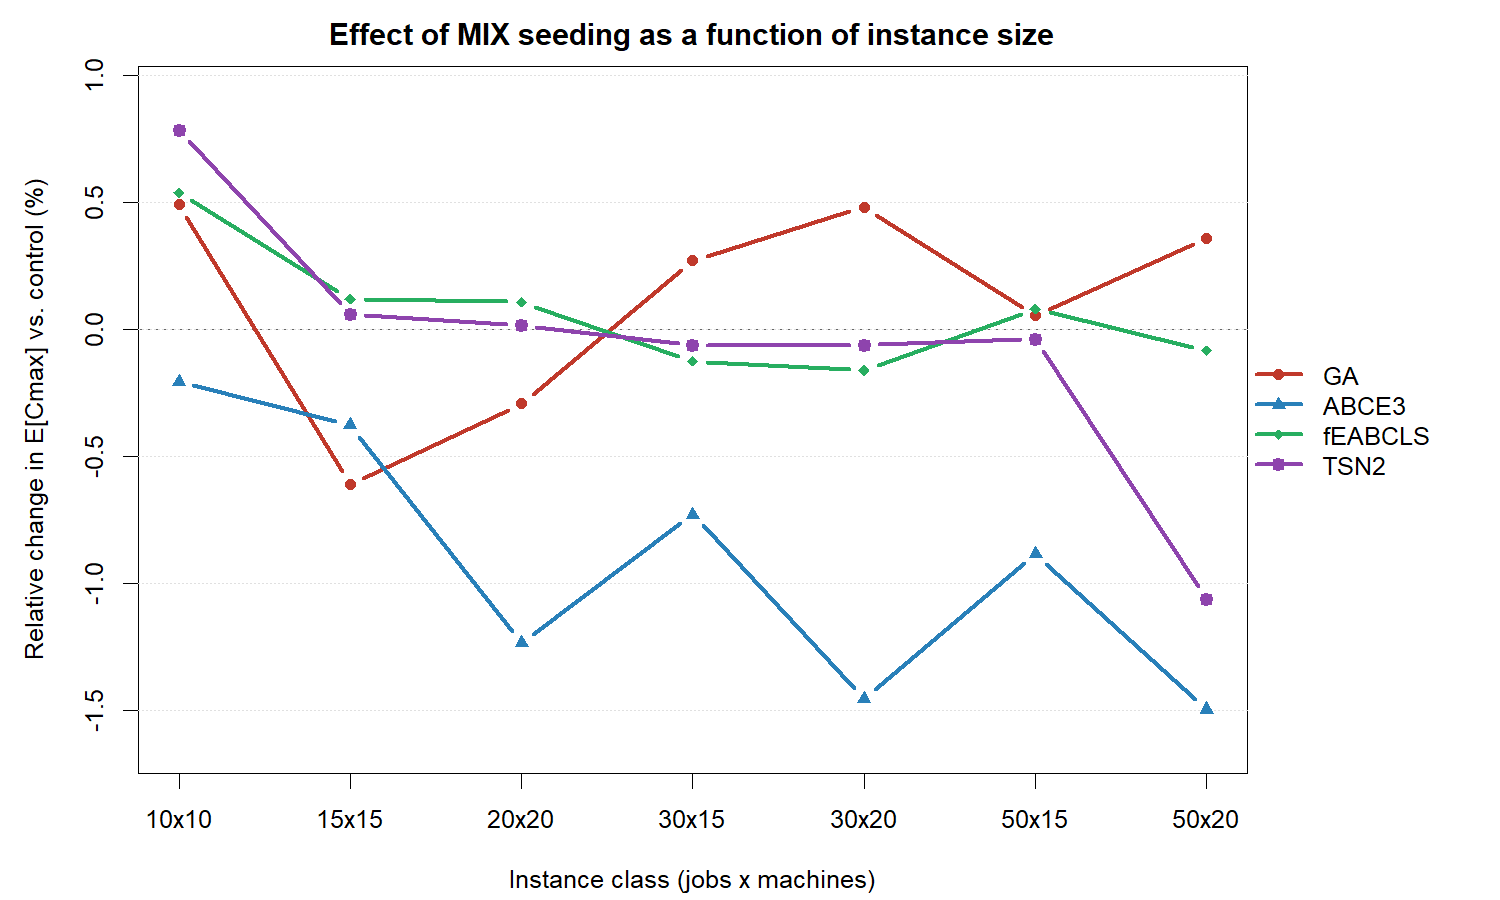
\includegraphics[width=\linewidth]{../figs/main_effect_by_size.png}
\caption{Relative change in $\mathbb{E}[C_{\max}]$ under MIX seeding with
respect to the unseeded control, by instance class (ordered by number of
operations). Negative values favour seeding. The benefit for ABCE3 and
TSN2 grows with instance size, whereas the penalty for the GA persists.}
\label{fig:size}
\end{figure}

Two trends emerge. For ABCE3 the gain deepens with size, from $-0.21\%$ on
the smallest instance to $-1.24\%$ on $20\times20$ and $-1.50\%$ on
$50\times20$. For TSN2 the effect is flat and near zero up to $50\times15$
and then drops sharply to $-1.06\%$ on $50\times20$ --- and on that class
\emph{every} seeded arm beats the control, including GP ($\Delta=-30.9$),
MOR ($\Delta=-25.6$) and GT ($\Delta=-19.6$), all three of which are
harmful everywhere else. The GA moves in the opposite direction, remaining
between $+0.05\%$ and $+0.48\%$ on the four largest classes.

Table~\ref{tab:tsn2class} makes the concentration explicit for TSN2, and it
is the single most important caveat in this paper. The ten $50\times20$
instances account for $94.8\%$ of the aggregate improvement; the remaining
51 instances contribute almost nothing. Reporting only the pooled figure of
Table~\ref{tab:rpd} would therefore misrepresent the result as a general
improvement of the state of the art, which it is not.

\begin{table}[t]
\centering
\caption{Decomposition of the MIX seeding effect on TSN2 by instance class.
$\Delta$ is the mean signed change in $\mathbb{E}[C_{\max}]$ (negative
favours seeding); the last column is each class's share of the total
improvement.}
\label{tab:tsn2class}
\begin{tabular}{lccccc}
\toprule
Class & $n$ & $\mathbb{E}[C_{\max}]$ A0 & $\mathbb{E}[C_{\max}]$ MIX & $\Delta$ (\%) & Share \\
\midrule
$10\times10$ & 1  & 937.1  & 944.5  & $+0.78$ & --- \\
$15\times15$ & 10 & 1253.6 & 1254.3 & $+0.06$ & --- \\
$20\times20$ & 10 & 1668.8 & 1669.1 & $+0.01$ & --- \\
$30\times15$ & 10 & 1844.8 & 1843.6 & $-0.06$ & 3.6\% \\
$30\times20$ & 10 & 2052.6 & 2051.4 & $-0.06$ & 3.4\% \\
$50\times15$ & 10 & 2780.3 & 2779.2 & $-0.04$ & 3.2\% \\
$\mathbf{50\times20}$ & 10 & \textbf{2970.1} & \textbf{2938.4} & $\mathbf{-1.06}$ & \textbf{94.8\%} \\
\bottomrule
\end{tabular}
\end{table}

The interpretation is a budget-starvation argument. On $50\times20$
instances (1000 operations) even a state-of-the-art tabu search cannot,
within the 900\,s cap, recover from a random start the structure that a
constructive heuristic supplies for free. Seeding does not make the search
better; it removes a phase of the search that the budget cannot afford.
This predicts that the benefit of seeding should be reported as a function
of the budget-to-size ratio rather than as a single aggregate figure, and
that published seeding gains obtained on small instances will not transfer.

\subsection{Anytime behaviour}\label{sec:res-anytime}

Final quality alone cannot distinguish a solver that is genuinely improved
by seeding from one that is merely given a head start. Because per-solver
budgets range from 60\,s to 900\,s across size classes, absolute time is
not comparable across instances; we therefore normalise each trace to the
fraction of its own budget consumed, the standard convention for aggregated
anytime curves, and average over instances on a common grid so that no
instance enters or leaves mid-curve. Figure~\ref{fig:anytimeall} shows the
resulting profiles over all 61 instances, and Table~\ref{tab:budgetfrac}
gives the values at five budget fractions.

\begin{figure}[t]
\centering
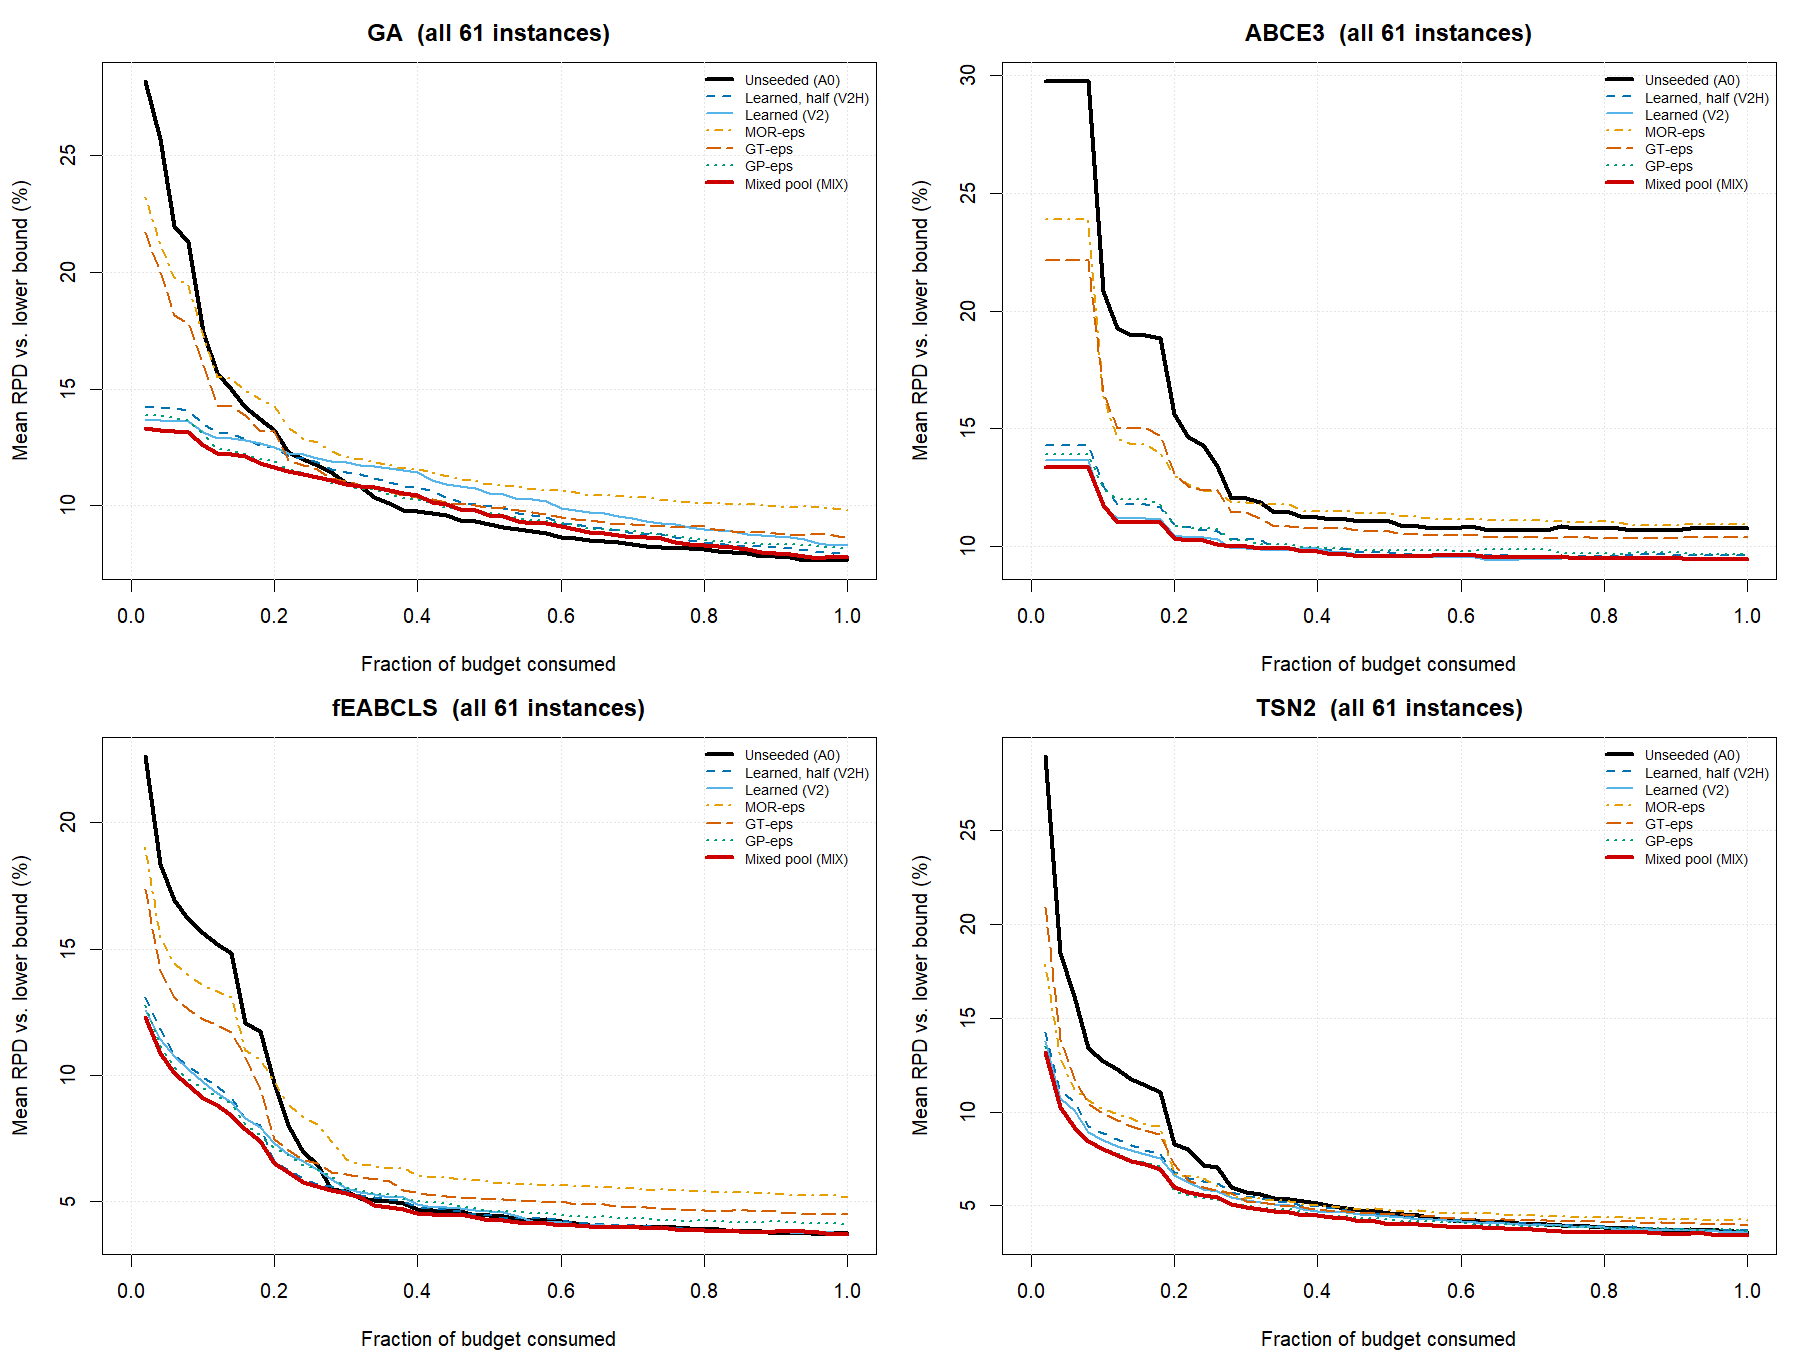
\includegraphics[width=\linewidth]{../figs/anytime_all.png}
\caption{Anytime behaviour over all 61 instances. Mean RPD with respect to
the published lower bound against the fraction of the per-instance budget
consumed, for the unseeded control and the two best seeded arms.}
\label{fig:anytimeall}
\end{figure}

\begin{table}[t]
\centering
\caption{Mean RPD (\%) over all 61 instances at five fractions of the
per-instance budget. Values are resampled from execution traces and agree
with Table~\ref{tab:rpd} to within the trace sampling resolution.}
\label{tab:budgetfrac}
\small
\begin{tabular}{llccccc}
\toprule
Solver & Arm & 10\% & 25\% & 50\% & 75\% & 100\% \\
\midrule
\multirow{7}{*}{GA}
 & A0  & 17.41 & 11.97 & \textbf{9.19} & \textbf{8.22} & \textbf{7.71} \\
 & V2H & 13.50 & 12.02 & 9.97  & 8.75  & 7.94 \\
 & V2  & 13.15 & 12.20 & 10.53 & 9.25  & 8.29 \\
 & MOR & 17.30 & 12.86 & 10.90 & 10.24 & 9.80 \\
 & GT  & 16.01 & 11.72 & 9.89  & 9.10  & 8.64 \\
 & GP  & 13.07 & 11.37 & 9.68  & 8.76  & 8.14 \\
 & MIX & \textbf{12.60} & \textbf{11.36} & 9.60 & 8.60 & 7.78 \\
\midrule
\multirow{7}{*}{ABCE3}
 & A0  & 20.83 & 14.30 & 11.05 & 10.86 & 10.78 \\
 & V2H & 12.54 & 10.67 & 9.76  & 9.56  & 9.64 \\
 & V2  & \textbf{11.71} & 10.38 & 9.64 & 9.51 & 9.52 \\
 & MOR & 16.39 & 12.38 & 11.41 & 11.06 & 10.96 \\
 & GT  & 16.49 & 12.40 & 10.66 & 10.40 & 10.39 \\
 & GP  & 12.49 & 10.79 & 9.86  & 9.72  & 9.69 \\
 & MIX & 11.73 & \textbf{10.27} & \textbf{9.57} & \textbf{9.58} & \textbf{9.46} \\
\midrule
\multirow{7}{*}{fEABCLS}
 & A0  & 15.64 & 6.94 & 4.47 & 3.97 & 3.75 \\
 & V2H & 9.91  & 5.92 & 4.47 & 3.97 & 3.74 \\
 & V2  & 9.74  & 6.62 & 4.61 & 3.97 & \textbf{3.68} \\
 & MOR & 13.57 & 8.34 & 5.80 & 5.48 & 5.17 \\
 & GT  & 12.24 & 6.69 & 5.08 & 4.72 & 4.48 \\
 & GP  & 9.49  & 6.42 & 4.62 & 4.27 & 4.06 \\
 & MIX & \textbf{9.10} & \textbf{5.77} & \textbf{4.26} & 3.97 & 3.71 \\
\midrule
\multirow{7}{*}{TSN2}
 & A0  & 12.70 & 7.17 & 4.60 & 3.98 & 3.60 \\
 & V2H & 8.86  & 6.29 & 4.48 & 3.95 & 3.69 \\
 & V2  & 8.47  & 5.88 & 4.45 & 3.95 & 3.64 \\
 & MOR & 10.14 & 6.44 & 4.75 & 4.46 & 4.25 \\
 & GT  & 9.95  & 5.97 & 4.54 & 4.19 & 3.98 \\
 & GP  & 8.06  & \textbf{5.41} & 4.29 & 3.89 & 3.65 \\
 & MIX & \textbf{8.00} & 5.56 & \textbf{4.04} & \textbf{3.64} & \textbf{3.44} \\
\bottomrule
\end{tabular}
\end{table}

The aggregate view exposes a result that final-quality tables cannot show:
\emph{at short budgets seeding is a large win for every solver in the
portfolio, including those for which it is worthless at convergence}. At
10\% of budget, MIX cuts mean RPD from 20.83\% to 11.73\% on ABCE3, from
15.64\% to 9.10\% on fEABCLS, from 17.41\% to 12.60\% on the GA and from
12.70\% to 8.00\% on TSN2 --- reductions of 44\%, 42\%, 28\% and 37\%
respectively. Yet by 100\% of budget fEABCLS has closed the gap entirely
($3.75\%$ vs.\ $3.71\%$) and the GA has overtaken its seeded arms. The
practical reading is that the question ``does seeding help?'' is ill-posed
unless the budget is specified: for a practitioner who can afford only a
tenth of our budget, seeding is decisive for all four solvers, including
the one it demonstrably harms at convergence.

The GA panel isolates the reversal. Its seeded arms lead until roughly
20\% of the budget, after which the control crosses and stays below to the
end. This is the anytime signature of the consolidation failure analysed in
Section~\ref{sec:whyga}: the seeded population is ahead while quality is
inherited from the seeds, and falls behind as soon as progress must come
from recombination. ABCE3 shows the opposite profile, a gap that opens
immediately and never closes.

The generator ranking is also stable along the whole trajectory, not merely
at the end. MOR is the uppermost seeded curve in all four panels and GT the
next, so their disadvantage is not an artefact of where measurement stops:
on the two ABC variants these pools are worse than the control at every
budget. MIX is the lowest curve in three of four panels for essentially the
entire run. Two observations qualify the ranking. First, GP and V2 are
competitive with MIX at very short budgets --- on TSN2 at 10\% of budget GP
reaches 8.06\% against MIX's 8.00\%, and on ABCE3 V2 reaches 11.71\%
against MIX's 11.73\%, i.e.\ marginally ahead --- so the advantage of the
mixed pool \emph{emerges as the search proceeds} rather than being
inherited from higher initial seed quality. That is exactly what one
expects if the operative variable is pool diversity rather than seed
quality, and Section~\ref{sec:res-seedqual} confirms it directly. Second,
V2 degrades relative to V2H on the GA as the budget grows (8.29\% versus
7.94\% at convergence), a hint that seeding the entire population with a
single learned policy is worse than seeding half of it, and that some
random material is worth retaining.

Figure~\ref{fig:anytime} restricts the same analysis to the $50\times20$
class in absolute time, where the seeding effect on the strong solvers is
concentrated.

\begin{figure}[t]
\centering
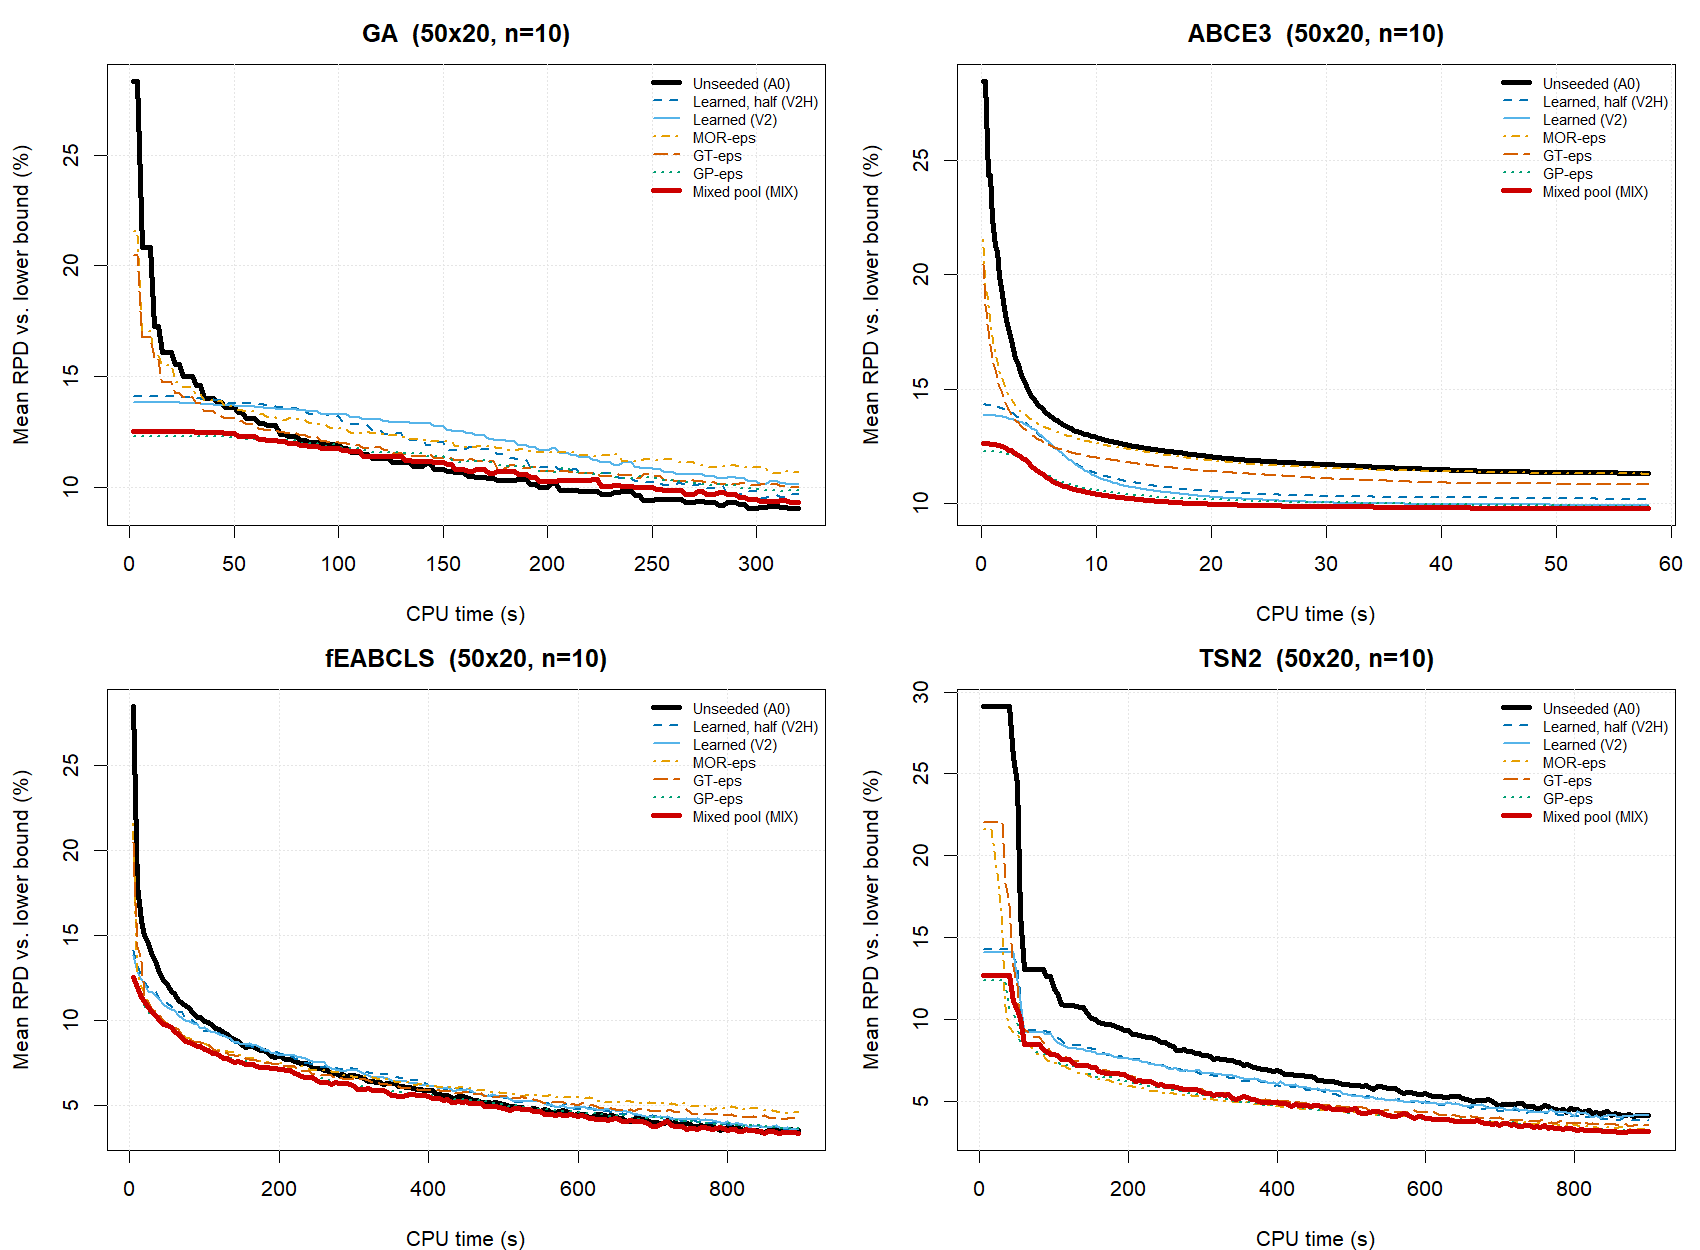
\includegraphics[width=\linewidth]{../figs/anytime_50x20.png}
\caption{Convergence on the $50\times20$ class (10 instances, 30 runs).
Mean RPD with respect to the published lower bound against CPU time, for
the unseeded control and the two best seeded arms. Note the differing time
axes: solver budgets are calibrated per solver and size class.}
\label{fig:anytime}
\end{figure}

Two features are specific to this class. ABCE3's control flattens at
approximately 11.2\% while both seeded arms flatten near 9.7\%, a gap
present from the first seconds that never closes --- a genuine improvement
in converged quality rather than an acceleration. TSN2's control exhibits a
sharp step near 50\,s, when the tabu phase first engages, and thereafter
descends steadily; MIX remains below it over the entire trajectory and is
still below at the budget limit (approximately 3.3\% against 4.1\%). The
separation is therefore not an artefact of where the budget stops.

One methodological consequence deserves emphasis. The GA result would have
been reported as a \emph{success} under any budget shorter than its
crossover point, which is precisely the artefact documented in
Section~\ref{sec:pilot}. Since seeding studies commonly fix a budget
without verifying convergence, this is a plausible source of optimistic
seeding claims in the literature, and it argues for reporting anytime
profiles rather than single-budget summaries.

\subsection{Time to target}\label{sec:res-ttt}

Anytime curves show \emph{that} seeded arms lead early; time-to-target
quantifies \emph{by how much}. We report the two metrics of
Section~\ref{sec:pilot}: (A) the time to come within 1\% of the arm's own
final value, and (B) the time to reach the unseeded control's final quality
within $+0.5\%$. Both are expressed as a fraction of the per-instance
budget so that classes with different budgets can be pooled, and both are
medians over the 61 instances. Metric B is reported together with the
proportion of instances on which the arm reaches the target at all, since a
median computed only over successes is meaningless without it.

\begin{table}[t]
\centering
\caption{Time to target, as a median fraction of the per-instance budget.
A: to within 1\% of the arm's own final value. B: to the unseeded control's
final quality $+0.5\%$. ``Reach'' is the percentage of the 61 instances on
which target B is attained; the median for B is taken over those instances
only.}
\label{tab:ttt}
\small
\begin{tabular}{llccc}
\toprule
Solver & Arm & A & B & Reach \\
\midrule
\multirow{4}{*}{GA}
 & A0  & 84\% & 86\% & 100\% \\
 & V2  & 87\% & 70\% & 41\% \\
 & MOR & 81\% & 87\% & \textbf{3\%} \\
 & MIX & 86\% & 70\% & 59\% \\
\midrule
\multirow{4}{*}{ABCE3}
 & A0  & 37\% & 37\% & 100\% \\
 & V2  & 40\% & 19\% & 98\% \\
 & MOR & 50\% & 37\% & 67\% \\
 & MIX & 37\% & \textbf{10\%} & 93\% \\
\midrule
\multirow{4}{*}{fEABCLS}
 & A0  & 59\% & 61\% & 100\% \\
 & V2  & 73\% & 46\% & 72\% \\
 & MOR & 72\% & 59\% & 10\% \\
 & MIX & 64\% & 41\% & 67\% \\
\midrule
\multirow{4}{*}{TSN2}
 & A0  & 76\% & 76\% & 100\% \\
 & V2  & 71\% & 63\% & 72\% \\
 & MOR & 55\% & 47\% & 31\% \\
 & MIX & 65\% & 55\% & 80\% \\
\bottomrule
\end{tabular}
\end{table}

Metric A discriminates almost nothing: every arm of every solver plateaus
between 55\% and 87\% of its budget, and the seeded arms of the GA appear
to plateau \emph{later} than the control. This is the expected behaviour of
a self-referential target --- an arm that settles quickly on a poor value
scores well --- and we report it mainly to document that it should not be
used alone.

Metric B, read together with the reach column, is informative. On ABCE3
the mixed pool attains the control's \emph{final} quality after 10\% of the
budget, a $3.6\times$ acceleration, and does so on 93\% of instances; V2
and GP achieve $2\times$ on 98\% and 93\%. These are genuine
``same quality, sooner'' results, and they are consistent with the
converged-quality finding for that solver. On TSN2 and fEABCLS the mixed
pool reaches the control's final quality at 55\% and 41\% of budget on 80\%
and 67\% of instances respectively --- a real but smaller acceleration.

The GA illustrates why the reach column is indispensable. Its seeded arms
appear to accelerate by 15--28\%, but they attain the control's final
quality on only 28--59\% of instances; MOR shows the extreme case, a median
of 87\% of budget computed over the 3\% of instances where it succeeds at
all. Quoting metric B alone would report an acceleration for arms that, on
most instances, never reach the target. Under this reading the GA has no
seeded arm that is faster to the control's quality on a majority of
instances, which is the anytime counterpart of its converged-quality loss.

\subsection{Initial-population quality: the mixed pool does not start
better}\label{sec:res-seedqual}

The obvious explanation for MIX's advantage would be that its seeds are
simply better. They are not. Table~\ref{tab:seedqual} reports the quality
of the initial population each arm actually receives, read from the
step-zero record of the traces, so it is the solvers' own evaluation rather
than the value stored with the pool.

\begin{table}[t]
\centering
\caption{Quality of the seeded initial population relative to the unseeded
control, averaged over five instances spanning $20\times20$ to
$50\times20$ (TSN2 traces). Negative is better. ``Mean'' is over all 250
initial individuals and is the quantity that characterises the pool.}
\label{tab:seedqual}
\begin{tabular}{lcc}
\toprule
Arm & Best individual & Mean of the 250 \\
\midrule
V2H & $-11.34\%$ & $-7.35\%$ \\
V2  & $-11.84\%$ & $-14.73\%$ \\
MOR & $-5.28\%$  & $-10.40\%$ \\
GT  & $-4.75\%$  & $-8.85\%$ \\
GP  & $\mathbf{-12.09\%}$ & $\mathbf{-15.48\%}$ \\
MIX & $-12.25\%$ & $-13.12\%$ \\
\bottomrule
\end{tabular}
\end{table}

On the mean of the initial population --- the natural measure of pool
quality --- MIX is \emph{worse} than both V2 and GP, by 1.6 and 2.4
percentage points respectively, and it never holds the best individual by a
meaningful margin. It nonetheless finishes ahead of both
(Table~\ref{tab:rpd}). A pool that starts worse and ends better is direct
evidence that the operative variable is composition, not seed quality.

This also disposes of a possible confound. The mixed pool is assembled from
exactly the same 1{,}024 solutions per generator that feed the V2, GT and
GP arms --- it introduces no new material, only a different mixture --- so
no difference in provenance or generation effort can be invoked to explain
its advantage.

\subsection{Which seeding strategy? Generator ranking and its
solver-dependence}\label{sec:res-ranking}

The practitioner's question is not whether seeding helps in general but
which pool to use, and whether that choice must be re-made for every
solver. We answer both with a Friedman test over the seven arms with the 61
instances as blocks, followed by Holm-corrected paired post-hoc
comparisons against the top-ranked arm of each solver.
Table~\ref{tab:ranking} reports the mean ranks.

\begin{table}[t]
\centering
\caption{Mean Friedman ranks of the seven arms (1 = best) over 61
instances. Friedman rejects rank equality for every solver
($p<10^{-15}$ throughout). Boldface marks arms not significantly worse
than that solver's top-ranked arm (Holm-corrected paired Wilcoxon,
$\alpha=0.05$).}
\label{tab:ranking}
\begin{tabular}{lccccccc}
\toprule
Solver & A0 & V2H & V2 & MOR & GT & GP & MIX \\
\midrule
GA      & \textbf{2.69} & \textbf{3.08} & 4.25 & 6.41 & 4.77 & 3.85 & \textbf{2.95} \\
ABCE3   & 5.60 & \textbf{3.08} & \textbf{2.50} & 6.14 & 4.96 & 3.31 & \textbf{2.41} \\
fEABCLS & \textbf{2.99} & \textbf{2.93} & \textbf{3.04} & 6.52 & 5.51 & 4.24 & \textbf{2.78} \\
TSN2    & 3.40 & 3.93 & 3.80 & 5.37 & 5.07 & 3.85 & \textbf{2.57} \\
\midrule
$\chi^2$ (df 6) & \multicolumn{7}{c}{GA 132.6 \quad ABCE3 185.0 \quad
fEABCLS 177.6 \quad TSN2 75.5} \\
\bottomrule
\end{tabular}
\end{table}

Two findings follow, and they answer different questions.

\paragraph{Which generator: the answer does not depend on the solver.}
The ranking of the six seeded arms is highly consistent across the
portfolio: restricted to those arms, the mean pairwise Spearman correlation
between the four rank vectors is $\rho=0.88$. MIX is the best
\emph{seeded} arm for all four solvers, with ranks between 2.41 and 2.95,
and is never significantly worse than the top-ranked arm of any solver ---
indeed it is the top-ranked arm outright for three of the four. MOR is last
for all four (5.37 to 6.52) and GT second-to-last for three. A practitioner
therefore does not need to re-tune the choice of generator per algorithm:
use a mixed pool, avoid the low-diversity constructive pools.

\paragraph{Whether to seed at all: the answer does depend on the solver.}
The only arm whose rank moves substantially across solvers is the unseeded
control, from 2.69 on the GA (where it is the top-ranked arm overall) to
5.60 on ABCE3 (where it ranks sixth of seven, beaten by every seeded arm
except MOR). Including A0 drags the mean pairwise agreement down from
$\rho=0.88$ to $\rho=0.69$, and the weakest pair, GA versus ABCE3, rises
from $\rho=0.36$ to $\rho=0.83$ once the control is removed. The
displacement of A0 is thus the entire source of cross-solver disagreement.

This dissociation is the cleanest statement of the paper's result. The
question ``which seeds are good?'' has a solver-independent answer, because
it is a property of the pool. The question ``should I seed?'' does not,
because it depends on whether the solver's variation operators can exploit
the pool --- the mechanism analysed in Section~\ref{sec:whyga}. Reporting
only the first, as seeding studies commonly do, produces a recommendation
that silently fails on solvers like the GA.

\paragraph{Why the advantage is not an artefact of sampling.} A natural
objection is that MIX might win because it exposes the search to more
distinct seed material. Three properties of the design rule this out. The
five pools are the same size ($L=1024$), so every arm draws 30 blocks of
250 under the same arithmetic. The mixed pool is assembled from precisely
the solutions that feed the V2, GT and GP arms, so it contains no material
those arms do not also see. And directly measured
(Section~\ref{sec:res-seedqual}), the population MIX actually receives is
on average \emph{worse} than the ones V2 and GP receive, yet it converges
to better solutions. Sampling breadth and seed quality both point the wrong
way for the objection; within-population generator diversity is what
remains.

\subsection{A limitation of CPU-time budgets}\label{sec:res-budget}

The stopping rule is a fixed CPU-time budget, measured with the process
clock. CPU-seconds are reproducible; the \emph{work} they buy is not,
because the instructions retired per CPU-second depend on contention for
cache and memory bandwidth among the concurrently executing workers. All
cells here were produced under an identical occupancy --- fourteen
concurrent workers throughout --- so the effect is constant across the
design, and within a solver it is in any case common to all seven arms,
leaving the paired instance-level comparisons that carry every claim in
this paper unaffected. What is \emph{not} transferable is the absolute
level: an RPD of 3.41\% for TSN2 is specific to this machine at this
occupancy and should not be compared against figures published for these
solvers elsewhere. More generally, studies reporting a single absolute
quality figure under a wall-clock or CPU-time budget, without stating the
hardware occupancy under which it was obtained, are less reproducible than
they appear.

\subsection{Threats addressed by design}\label{sec:res-threats}

Three checks guard the numbers above. First, expected makespans were
recomputed from the stored chromosomes with an independent decoder
implementation (insertion SGS, componentwise maximum) over 3255 solutions
spanning all four solvers, all seven arms and one instance from each size
class. In 3250 cases the reported interval makespan is reproduced exactly.
The five exceptions, all on $50\times15$ and $50\times20$ instances, differ
in one interval endpoint only and always in the same direction: the
re-decoded schedule is \emph{better} than the recorded one, by between 0.5
and 3.5 units of $\mathbb{E}[C_{\max}]$ on values near 3100, i.e.\ at most
$0.11\%$. This is expected rather than anomalous --- the active-schedule
builder can improve marginally on the schedule an algorithm actually held
at termination --- and it means the figures we report are, in $0.15\%$ of
cases, very slightly pessimistic. No discrepancy runs in the optimistic
direction. Second, all arms within an instance share the RNG stream, so
the paired tests compare like with like. Third, the stopping rule is a
fixed CPU-time budget per size class, identical across arms, which
eliminates the stagnation-triggered artefact documented in
Section~\ref{sec:pilot}.

\section{Discussion}\label{sec:discussion}

\subsection{Seeding quality is not the operative variable}

The pre-registered hypothesis --- that seeding helps precisely those
solvers whose own search saturates below the seed level --- is not
supported. Ordering the portfolio by unseeded RPD gives ABCE3 (10.51) $>$
GA (7.52) $>$ fEABCLS (3.67) $>$ TSN2 (3.60), but the seeding effect
follows the order ABCE3 (large gain) $>$ TSN2 (small gain) $>$ fEABCLS
(null) $>$ GA (loss). The strongest solver in the portfolio benefits while
a mid-ranked one is harmed, so solver quality alone does not predict the
sign of the effect.

What does predict it is the interaction between the seeds and the
solver's variation operators. MIX --- equal thirds of v2, GT and GP, i.e.\
84/83/83 of the 250 seeded individuals --- is the best or joint-best arm
everywhere, while the single-generator pools of comparable individual
quality (V2, GP) are weaker and the low-diversity pools (MOR, GT) are
actively harmful. A pool of near-identical high-quality schedules narrows
the region the operators explore; a pool that is good \emph{and} varied
does not.

\subsection{Why the genetic algorithm is harmed: a failure to
consolidate}\label{sec:whyga}

The intuitive explanation for a seeding-induced loss is premature
convergence: a population of good, similar individuals collapses onto a
local optimum. The data do not support it. We instrumented the GA and
ABCE3 with the mean pairwise Hamming distance of the population, sampled
every 10\,s over 10 runs on four medium instances (normalised to $[0,1]$,
where 0 denotes an identical population). Table~\ref{tab:hamming} reports
the result. The seeded GA is not less diverse than its control --- it is
\emph{significantly more} diverse, by $+24.3\%$ under V2 and $+13.7\%$
under MIX (paired Wilcoxon, $p<10^{-4}$), and it ends the run at $0.720$
against the control's $0.464$.

\begin{table}[t]
\centering
\caption{Mean pairwise Hamming distance of the population (0 = identical
population, 1 = maximal positional difference), averaged over four
instances and 10 runs. The seeded GA converges structurally \emph{less}
than its control; ABCE3 is unaffected by seeding.}
\label{tab:hamming}
\begin{tabular}{llcccc}
\toprule
Solver & Arm & Start & Mean & End & Drop \\
\midrule
\multirow{3}{*}{GA}
 & A0  & 0.9474 & 0.7646 & 0.4639 & $-51.0\%$ \\
 & V2  & 0.9310 & 0.8845 & 0.7195 & $-22.7\%$ \\
 & MIX & 0.9301 & 0.8350 & 0.5552 & $-40.3\%$ \\
\midrule
\multirow{3}{*}{ABCE3}
 & A0  & 0.9474 & 0.7140 & 0.8541 & $-9.9\%$ \\
 & V2  & 0.9310 & 0.7059 & 0.8602 & $-7.6\%$ \\
 & MIX & 0.9301 & 0.7171 & 0.8497 & $-8.6\%$ \\
\bottomrule
\end{tabular}
\end{table}

The failure is therefore the opposite of premature convergence: within a
fixed budget the seeded GA never consolidates. Its control contracts by
$51.0\%$ in structural spread and exploits the region it has found; under
V2 the seeded variant contracts by only $22.7\%$ and is still exploring
when the budget expires. The proximate cause is that the seeds, being
drawn from generators with different construction logic, are good but
mutually \emph{dissimilar}; JOX recombining two structurally divergent
parents produces offspring that inherit the operation ordering of neither,
so selection cannot accumulate structure. The harm grows with instance size
(Section~\ref{sec:res-size}) because longer chromosomes need more
generations to consolidate, and the budget does not grow proportionally.

The contrast with ABCE3 supports this reading. Seeding does not perturb
ABCE3's diversity trajectory at all (differences of $-2.3\%$ and $+4.0\%$,
$p=0.27$ and $p=0.90$), and its population stays dispersed throughout
($0.85$ at the end). ABCE3 does not rely on recombining population members
to build structure, so seeds are retained and refined rather than
destroyed. The determining factor is thus not seed quality but whether the
solver's variation operator can exploit structurally heterogeneous parents.

The ordering of the two seeded arms is itself informative. V2, drawn from a
single generator, produces the least consolidation ($-22.7\%$) and the
largest loss in final quality; MIX, despite being the more heterogeneous
pool, consolidates further ($-40.3\%$) and is the better of the two arms on
this solver. Structural heterogeneity of the \emph{pool} and structural
heterogeneity of the \emph{surviving population} are therefore not the same
quantity: what obstructs the GA is a population the operator cannot
consolidate, not a diverse pool as such.

\subsection{Practitioner guidance}

The results support three concrete recommendations. (i) Seed with a
\emph{mixed} pool; the cost of running three generators instead of one is
negligible relative to the search budget and it dominates every
single-generator pool tested. (ii) Expect gains to grow with the
size-to-budget ratio: on small instances seeding is at best neutral for
strong solvers. (iii) Verify operator compatibility before seeding a
recombination-based algorithm; a null or negative result there is not a
failure of the seeds but a mismatch with the variation operator.

\subsection{Limitations}

The study covers one problem family (interval JSP) and one encoding
(permutation with repetition), so the operator-compatibility argument of
Section~\ref{sec:discussion} is a hypothesis supported by an internal
contrast, not an independently tested claim. Budgets are wall-clock
CPU-time caps on a single machine; while all arms within a cell share the
same cap, absolute times are not portable. Finally, the training cost of
the learned policy is excluded from the per-run budget, on the grounds that
it is amortised across all instances --- a reasonable but not neutral
accounting choice, which we report explicitly rather than absorb.

\section{Conclusions}\label{sec:conclusions}

We conducted, to our knowledge, the largest controlled study of population
seeding for the interval job shop: 4 published solvers, 7 initialisation
arms, 61 benchmark instances and 30 paired runs per cell, evaluated against
published lower bounds under a fixed-budget protocol designed to eliminate
three artefacts we document in a pilot study.

Seeding is not uniformly beneficial, and its sign is not predicted by
solver strength. A mixed pool improves the weakest solver by a wide margin
(35 wins, 0 losses out of 61), improves the state-of-the-art tabu hybrid
measurably (15--5, RPD 3.60\% $\rightarrow$ 3.41\%), leaves a memetic ABC
unchanged, and \emph{degrades} a genetic algorithm that cannot consolidate
structurally heterogeneous parents. The benefit grows with the ratio of
instance size to search budget, to the point where on the largest class
every generator we tested --- including those harmful elsewhere ---
improves the state of the art. Under the Friedman ranking the mixed pool is
the best arm for three of the four solvers and statistically
indistinguishable from the best on the fourth, so the choice of generator,
unlike the decision to seed at all, does not have to be revisited per
algorithm.

The practical consequence is that seeding should be treated as an
interaction between pool composition and variation operator, evaluated at
the budget and instance size of the intended application, rather than as a
property of the seeds alone.

%% =========================================================================
\section*{Data and code availability}
%% Corrected pools, seeding operator, setups, run logs, aggregated CSVs and
%% analysis scripts to be deposited on Zenodo (group practice). Commit hash
%% of the solver framework to be pinned at submission.

\bibliographystyle{elsarticle-num}
\bibliography{references}

\end{document}
